\documentclass{beamer}
\usepackage{relsize}
\usepackage{color}

\usepackage{listings}
\usetheme{CambridgeUS}
%\usepackage{beamerthemesplit} % new 
\usepackage{enumitem}
\usepackage{amsmath}                    % See geometry.pdf to learn the layout options. 
\usepackage{amsthm}                   % See geometry.pdf to learn the layout options. There 
\usepackage{amssymb}                    % See geometry.pdf to learn the layout options. 
\usepackage[utf8]{inputenc} 
\usepackage{graphicx}
\usepackage[english,bulgarian]{babel}
\usepackage[framemethod=tikz]{mdframed}
\usepackage{caption}
\usepackage{tikz}
\usepackage{forest}
\usetikzlibrary{shapes,arrows,positioning,calc,chains}

\lstset{language=C++,
                basicstyle=\ttfamily,
                keywordstyle=\color{blue}\ttfamily,
                stringstyle=\color{red}\ttfamily,
                commentstyle=\color{green}\ttfamily,
                morecomment=[l][\color{magenta}]{\#}
}

\newtheorem{mydef}{Дефиниция}[section]
\newtheorem{lem}{Лема}[section]
\newtheorem{thm}{Твърдение}[section]

\DeclareMathOperator{\restrict}{\upharpoonright}

\setitemize{label=\usebeamerfont*{itemize item}%
  \usebeamercolor[fg]{itemize item}
  \usebeamertemplate{itemize item}}

\setbeamercovered{transparent}

\captionsetup{font=footnotesize}

\lstset{breaklines=true}
\tikzset{
block/.style = {draw, fill=white, rectangle,align = center},
entry/.style = {draw, fill=black, circle, radius=3em},
condition/.style = {draw, fill=white, diamond, align = center,node distance=3cm},
fork/.style = {draw, fill=black, circle,inner sep=1pt},
lnode/.style={rectangle split, rectangle split parts=3,draw, rectangle split horizontal},
treenode/.style = {align=center, inner sep=0pt, text centered, circle, font=\sffamily\bfseries, draw=black, fill=white, text width=1.5em}
}


\begin{document}
\title[Структури от данни и програмиране]{Линейни двусвързани списъци и Skip List. Итератори} 
\author{Калин Георгиев} 
\frame{\titlepage} 

\section{Линейни двусвързани списъци} 


\begin{frame}
\centerline{Линейни двусвързани списъци}
\end{frame}


\begin{frame}[fragile]
\frametitle{Doubly Linked List}
\begin{figure}
  \centering

    \begin{tikzpicture}[auto, node distance=2cm,>=latex']
    \node[lnode] (n1) {\nodepart{two}1};
    \node[lnode, right of = n1] (n2) {\nodepart{two}2};
    \node[lnode, right of = n2] (n3) {\nodepart{two}3};
    \node[lnode, right of = n3] (n4) {\nodepart{two}4};
    \node[lnode, right of = n4] (n5) {\nodepart{two}5};

    \node[rectangle,left of = n1](start){};

    \draw[*->]  (start)-- (n1);

    \draw[*->] let \p1 = (n2.three), \p2 = (n1.center) in (\x1,\y2) -- (n3);
    \draw[*->] let \p1 = (n1.three), \p2 = (n1.center) in (\x1,\y2) -- (n2);
    \draw[*->] let \p1 = (n3.three), \p2 = (n1.center) in (\x1,\y2) -- (n4);
    \draw[*->] let \p1 = (n4.three), \p2 = (n1.center) in (\x1,\y2) -- (n5);
    \draw[*->,dashed] let \p1 = (n2.one), \p2 = (n1.center) in ([shift={(0.1cm,-0.1cm)}]\x1,\y2) |-([shift={(0,0.5cm)}]n2.north west) -- ([shift={(0,0.5cm)}]n1.north) -| ([shift={(-1cm,0cm)}]n1);
    \draw[*->,dashed] let \p1 = (n3.one), \p2 = (n2.center) in ([shift={(0.1cm,0.1cm)}]\x1,\y2) |-([shift={(0,-1cm)}]n3.north west) -- ([shift={(0,-1cm)}]n2.north) -| ([shift={(-1cm,0cm)}]n2);
    \draw[*->,dashed] let \p1 = (n4.one), \p2 = (n3.center) in ([shift={(0.1cm,-0.1cm)}]\x1,\y2) |-([shift={(0,0.5cm)}]n4.north west) -- ([shift={(0,0.5cm)}]n3.north) -| ([shift={(-1cm,0cm)}]n3);
    \draw[*->,dashed] let \p1 = (n5.one), \p2 = (n4.center) in ([shift={(0.1cm,0.1cm)}]\x1,\y2) |-([shift={(0,-1cm)}]n5.north west) -- ([shift={(0,-1cm)}]n4.north) -| ([shift={(-1cm,0cm)}]n4);
    \end{tikzpicture}
  \caption{Двусвързан списък}
  \label{fig:skiplist}
\end{figure}


\end{frame}

\section{Skip List} 

\begin{frame}
\centerline{Skip List}
\end{frame}


\begin{frame}[fragile]
\frametitle{Skip List (с две нива)}
\begin{figure}
  \centering

    \begin{tikzpicture}[auto, node distance=2cm,>=latex']
    \node[lnode] (n1) {\nodepart{two}1};
    \node[lnode, right of = n1] (n2) {\nodepart{two}2};
    \node[lnode, right of = n2] (n3) {\nodepart{two}3};
    \node[lnode, right of = n3] (n4) {\nodepart{two}4};
    \node[lnode, right of = n4] (n5) {\nodepart{two}5};

    \node[rectangle,left of = n1](start){};

    \draw[*->]  (start)-- (n1);

    \draw[*->] let \p1 = (n2.three), \p2 = (n1.center) in (\x1,\y2) -- (n3);
    \draw[*->] let \p1 = (n1.three), \p2 = (n1.center) in (\x1,\y2) -- (n2);
    \draw[*->] let \p1 = (n3.three), \p2 = (n1.center) in (\x1,\y2) -- (n4);
    \draw[*->] let \p1 = (n4.three), \p2 = (n1.center) in (\x1,\y2) -- (n5);
    \draw[*->,dashed] let \p1 = (n1.one), \p2 = (n1.center) in ([shift={(0.1cm,-0.1cm)}]\x1,\y2) |-([shift={(0,0.5cm)}]n1.north east) -- ([shift={(0,0.5cm)}]n3.north) -| (n3);
    \draw[*->,dashed] let \p1 = (n3.one), \p2 = (n3.center) in ([shift={(0.1cm,0.1cm)}]\x1,\y2) |-([shift={(0,-0.5cm)}]n3.south east) -- ([shift={(0,-0.5cm)}]n5.south) -| (n5);
    \end{tikzpicture}
  \caption{Списък с прескачане}
  \label{fig:skiplist}
\end{figure}

\end{frame}

\section{Итератори} 


\begin{frame}[fragile]
  \frametitle{Skip List (с повече нива)}
  \begin{figure}
    \centering
    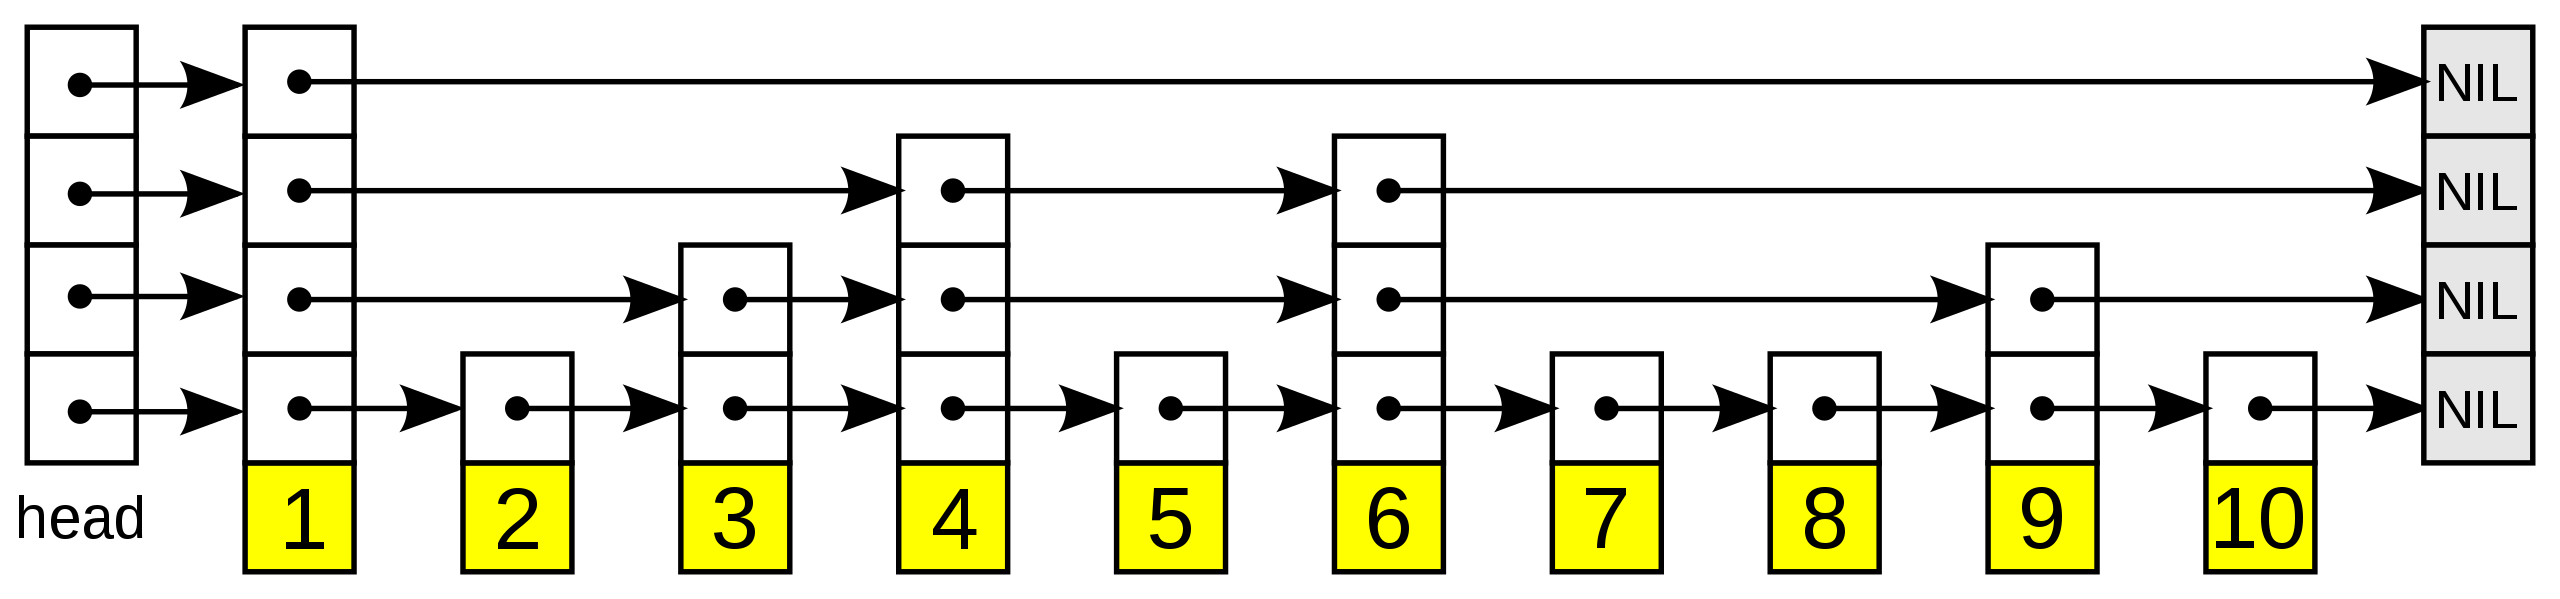
\includegraphics[width=10cm]{images/skiplist_wikipedia}
  
    \caption{SkipList с 4 нива. Източник: Wikipedia}
    \label{fig:tree1}
    \end{figure}  
\end{frame}
  


\begin{frame}
\centerline{Итератори}
\end{frame}

\begin{frame}[fragile]
  \frametitle{Приложение}

  Как достъпваме последователно (итерираме) елементите на контейнер?
  \begin{itemize}
    \item чрез индекс \\
          \verb#for (size_t i = 0; i < v.size(); ++i){...v[i]...}#
    \item \verb#for (T& x : container){...}#
  \end{itemize}
  Проблеми на простото индексиране:
  \begin{itemize}
    \item производителност
    \item понякога поредният номер е заблуждаващ
    \item не можем да се абстрахираме от контейнера\\
    \verb#void map (T (*f) (const T&), [....] WHAT)#
  \end{itemize}
  
  
  \end{frame}

  
  \begin{frame}[fragile]
    \frametitle{``Речник'' на линейното обхождане}
  
    \verb#for (size_t i = 0; i < v.size(); ++i){...v[i]...}#

    \begin{itemize}
      \item Започни!
      \item Дай следващия (предишния)!
      \item Има ли още?
    \end{itemize}
    \verb#>for (size_t j = 0; j < v.size(); ++j){if (i==j)...}#   
    \begin{itemize}
      \item Тези позиции еднакви ли са?
    \end{itemize}
  \end{frame}
  


\begin{frame}[fragile]
\frametitle{Итератори}

Създаване на итератор в контейнерния клас:
\begin{itemize}
  \item \texttt{begin}
  \item \texttt{end}
\end{itemize}
Операции с итератора
\begin{itemize}
  \item \texttt{*}
  \item ++, -{}-
  \item == (\emph{Итератор към ``края''})
  \item копиране
  \item \texttt{for}
\end{itemize}


\end{frame}


\begin{frame}
\centerline{Благодаря за вниманието!}
\end{frame}


\end{document}

\begin{columns}[t]
  \begin{column}{0.55\textwidth}

  \end{column}
  \begin{column}{0.45\textwidth}

  \end{column}
\end{columns}


